\documentclass[twoside]{book}

% Packages required by doxygen
\usepackage{fixltx2e}
\usepackage{calc}
\usepackage{doxygen}
\usepackage[export]{adjustbox} % also loads graphicx
\usepackage{graphicx}
\usepackage[utf8]{inputenc}
\usepackage{makeidx}
\usepackage{multicol}
\usepackage{multirow}
\PassOptionsToPackage{warn}{textcomp}
\usepackage{textcomp}
\usepackage[nointegrals]{wasysym}
\usepackage[table]{xcolor}

% Font selection
\usepackage[T1]{fontenc}
\usepackage[scaled=.90]{helvet}
\usepackage{courier}
\usepackage{amssymb}
\usepackage{sectsty}
\renewcommand{\familydefault}{\sfdefault}
\allsectionsfont{%
  \fontseries{bc}\selectfont%
  \color{darkgray}%
}
\renewcommand{\DoxyLabelFont}{%
  \fontseries{bc}\selectfont%
  \color{darkgray}%
}
\newcommand{\+}{\discretionary{\mbox{\scriptsize$\hookleftarrow$}}{}{}}

% Page & text layout
\usepackage{geometry}
\geometry{%
  a4paper,%
  top=2.5cm,%
  bottom=2.5cm,%
  left=2.5cm,%
  right=2.5cm%
}
\tolerance=750
\hfuzz=15pt
\hbadness=750
\setlength{\emergencystretch}{15pt}
\setlength{\parindent}{0cm}
\setlength{\parskip}{0.2cm}
\makeatletter
\renewcommand{\paragraph}{%
  \@startsection{paragraph}{4}{0ex}{-1.0ex}{1.0ex}{%
    \normalfont\normalsize\bfseries\SS@parafont%
  }%
}
\renewcommand{\subparagraph}{%
  \@startsection{subparagraph}{5}{0ex}{-1.0ex}{1.0ex}{%
    \normalfont\normalsize\bfseries\SS@subparafont%
  }%
}
\makeatother

% Headers & footers
\usepackage{fancyhdr}
\pagestyle{fancyplain}
\fancyhead[LE]{\fancyplain{}{\bfseries\thepage}}
\fancyhead[CE]{\fancyplain{}{}}
\fancyhead[RE]{\fancyplain{}{\bfseries\leftmark}}
\fancyhead[LO]{\fancyplain{}{\bfseries\rightmark}}
\fancyhead[CO]{\fancyplain{}{}}
\fancyhead[RO]{\fancyplain{}{\bfseries\thepage}}
\fancyfoot[LE]{\fancyplain{}{}}
\fancyfoot[CE]{\fancyplain{}{}}
\fancyfoot[RE]{\fancyplain{}{\bfseries\scriptsize Generated on Fri Feb 6 2015 13\+:10\+:31 for Queue\+Manager\+Atmel by Doxygen }}
\fancyfoot[LO]{\fancyplain{}{\bfseries\scriptsize Generated on Fri Feb 6 2015 13\+:10\+:31 for Queue\+Manager\+Atmel by Doxygen }}
\fancyfoot[CO]{\fancyplain{}{}}
\fancyfoot[RO]{\fancyplain{}{}}
\renewcommand{\footrulewidth}{0.4pt}
\renewcommand{\chaptermark}[1]{%
  \markboth{#1}{}%
}
\renewcommand{\sectionmark}[1]{%
  \markright{\thesection\ #1}%
}

% Indices & bibliography
\usepackage{natbib}
\usepackage[titles]{tocloft}
\setcounter{tocdepth}{3}
\setcounter{secnumdepth}{5}
\makeindex

% Hyperlinks (required, but should be loaded last)
\usepackage{ifpdf}
\ifpdf
  \usepackage[pdftex,pagebackref=true]{hyperref}
\else
  \usepackage[ps2pdf,pagebackref=true]{hyperref}
\fi
\hypersetup{%
  colorlinks=true,%
  linkcolor=blue,%
  citecolor=blue,%
  unicode%
}

% Custom commands
\newcommand{\clearemptydoublepage}{%
  \newpage{\pagestyle{empty}\cleardoublepage}%
}


%===== C O N T E N T S =====

\begin{document}

% Titlepage & ToC
\hypersetup{pageanchor=false,
             bookmarks=true,
             bookmarksnumbered=true,
             pdfencoding=unicode
            }
\pagenumbering{roman}
\begin{titlepage}
\vspace*{7cm}
\begin{center}%
{\Large Queue\+Manager\+Atmel }\\
\vspace*{1cm}
{\large Generated by Doxygen 1.8.9.1}\\
\vspace*{0.5cm}
{\small Fri Feb 6 2015 13:10:31}\\
\end{center}
\end{titlepage}
\clearemptydoublepage
\tableofcontents
\clearemptydoublepage
\pagenumbering{arabic}
\hypersetup{pageanchor=true}

%--- Begin generated contents ---
\chapter{Hierarchical Index}
\section{Class Hierarchy}
This inheritance list is sorted roughly, but not completely, alphabetically\+:\begin{DoxyCompactList}
\item \contentsline{section}{\+\_\+\+D\+E\+L\+A\+Y\+\_\+\+T\+A\+B\+L\+E}{\pageref{struct___d_e_l_a_y___t_a_b_l_e}}{}
\item \contentsline{section}{P\+Queue}{\pageref{class_p_queue}}{}
\item \contentsline{section}{Queue\+Manager}{\pageref{class_queue_manager}}{}
\item \contentsline{section}{S\+P\+I\+Class}{\pageref{class_s_p_i_class}}{}
\item Stream\begin{DoxyCompactList}
\item \contentsline{section}{Software\+Serial}{\pageref{class_software_serial}}{}
\end{DoxyCompactList}
\end{DoxyCompactList}

\chapter{Class Index}
\section{Class List}
Here are the classes, structs, unions and interfaces with brief descriptions\+:\begin{DoxyCompactList}
\item\contentsline{section}{\hyperlink{struct___d_e_l_a_y___t_a_b_l_e}{\+\_\+\+D\+E\+L\+A\+Y\+\_\+\+T\+A\+B\+L\+E} }{\pageref{struct___d_e_l_a_y___t_a_b_l_e}}{}
\item\contentsline{section}{\hyperlink{class_p_queue}{P\+Queue} }{\pageref{class_p_queue}}{}
\item\contentsline{section}{\hyperlink{class_queue_manager}{Queue\+Manager} }{\pageref{class_queue_manager}}{}
\item\contentsline{section}{\hyperlink{class_software_serial}{Software\+Serial} }{\pageref{class_software_serial}}{}
\item\contentsline{section}{\hyperlink{class_s_p_i_class}{S\+P\+I\+Class} }{\pageref{class_s_p_i_class}}{}
\end{DoxyCompactList}

\chapter{File Index}
\section{File List}
Here is a list of all documented files with brief descriptions\+:\begin{DoxyCompactList}
\item\contentsline{section}{{\bfseries P\+Queue.\+h} }{\pageref{_p_queue_8h}}{}
\item\contentsline{section}{{\bfseries Queue\+Manager.\+h} }{\pageref{_queue_manager_8h}}{}
\item\contentsline{section}{Arduino\+Libraries/\+Software\+Serial/{\bfseries Software\+Serial.\+h} }{\pageref{_software_serial_8h}}{}
\item\contentsline{section}{Arduino\+Libraries/\+S\+P\+I/{\bfseries S\+P\+I.\+h} }{\pageref{_s_p_i_8h}}{}
\item\contentsline{section}{src/config/\hyperlink{conf__board_8h}{conf\+\_\+board.\+h} \\*A\+Tmega2560 on S\+T\+K600 board configuration template }{\pageref{conf__board_8h}}{}
\item\contentsline{section}{Visual Micro/{\bfseries .\+Queue\+Manager\+Atmel.\+vsarduino.\+h} }{\pageref{_8_queue_manager_atmel_8vsarduino_8h}}{}
\end{DoxyCompactList}

\chapter{Class Documentation}
\hypertarget{struct___d_e_l_a_y___t_a_b_l_e}{}\section{\+\_\+\+D\+E\+L\+A\+Y\+\_\+\+T\+A\+B\+L\+E Struct Reference}
\label{struct___d_e_l_a_y___t_a_b_l_e}\index{\+\_\+\+D\+E\+L\+A\+Y\+\_\+\+T\+A\+B\+L\+E@{\+\_\+\+D\+E\+L\+A\+Y\+\_\+\+T\+A\+B\+L\+E}}
\subsection*{Public Attributes}
\begin{DoxyCompactItemize}
\item 
\hypertarget{struct___d_e_l_a_y___t_a_b_l_e_a81dc0c3fb2cc8893f4666f23f8db9eca}{}long {\bfseries baud}\label{struct___d_e_l_a_y___t_a_b_l_e_a81dc0c3fb2cc8893f4666f23f8db9eca}

\item 
\hypertarget{struct___d_e_l_a_y___t_a_b_l_e_a51aab1d8b68a8ea27646618a30b0e938}{}unsigned short {\bfseries rx\+\_\+delay\+\_\+centering}\label{struct___d_e_l_a_y___t_a_b_l_e_a51aab1d8b68a8ea27646618a30b0e938}

\item 
\hypertarget{struct___d_e_l_a_y___t_a_b_l_e_a8b81bfff2b179bdc4b6cd2f57df74e8f}{}unsigned short {\bfseries rx\+\_\+delay\+\_\+intrabit}\label{struct___d_e_l_a_y___t_a_b_l_e_a8b81bfff2b179bdc4b6cd2f57df74e8f}

\item 
\hypertarget{struct___d_e_l_a_y___t_a_b_l_e_a459c08839bc23ed1e22b146f7f3ce13d}{}unsigned short {\bfseries rx\+\_\+delay\+\_\+stopbit}\label{struct___d_e_l_a_y___t_a_b_l_e_a459c08839bc23ed1e22b146f7f3ce13d}

\item 
\hypertarget{struct___d_e_l_a_y___t_a_b_l_e_a20098fe273924c2456690a6ea96dc891}{}unsigned short {\bfseries tx\+\_\+delay}\label{struct___d_e_l_a_y___t_a_b_l_e_a20098fe273924c2456690a6ea96dc891}

\end{DoxyCompactItemize}


The documentation for this struct was generated from the following file\+:\begin{DoxyCompactItemize}
\item 
Arduino\+Libraries/\+Software\+Serial/Software\+Serial.\+cpp\end{DoxyCompactItemize}

\hypertarget{class_p_queue}{}\section{P\+Queue Class Reference}
\label{class_p_queue}\index{P\+Queue@{P\+Queue}}
\subsection*{Public Member Functions}
\begin{DoxyCompactItemize}
\item 
\hypertarget{class_p_queue_a3987253271078091d1986ca05a3164e4}{}void {\bfseries Insert} (Task\+Definition task\+Def, Task\+Base task, long priority)\label{class_p_queue_a3987253271078091d1986ca05a3164e4}

\end{DoxyCompactItemize}


The documentation for this class was generated from the following files\+:\begin{DoxyCompactItemize}
\item 
P\+Queue.\+h\item 
P\+Queue.\+cpp\end{DoxyCompactItemize}

\hypertarget{class_queue_manager}{}\section{Queue\+Manager Class Reference}
\label{class_queue_manager}\index{Queue\+Manager@{Queue\+Manager}}
\subsection*{Public Member Functions}
\begin{DoxyCompactItemize}
\item 
\hypertarget{class_queue_manager_a11e056b65033377927e14cc101a21c13}{}void {\bfseries Add\+Task} (Task\+Definition td, Task\+Base task)\label{class_queue_manager_a11e056b65033377927e14cc101a21c13}

\item 
\hypertarget{class_queue_manager_a85fda8e25818019f1f62cc29b7f7cd6d}{}Logger $\ast$ {\bfseries Get\+Logger} ()\label{class_queue_manager_a85fda8e25818019f1f62cc29b7f7cd6d}

\item 
\hypertarget{class_queue_manager_a66099fb771c3279a705c08558a3d9aa1}{}unsigned long {\bfseries Get\+Time} ()\label{class_queue_manager_a66099fb771c3279a705c08558a3d9aa1}

\end{DoxyCompactItemize}


The documentation for this class was generated from the following files\+:\begin{DoxyCompactItemize}
\item 
Queue\+Manager.\+h\item 
Queue\+Manager.\+cpp\end{DoxyCompactItemize}

\hypertarget{class_software_serial}{}\section{Software\+Serial Class Reference}
\label{class_software_serial}\index{Software\+Serial@{Software\+Serial}}
Inheritance diagram for Software\+Serial\+:\begin{figure}[H]
\begin{center}
\leavevmode
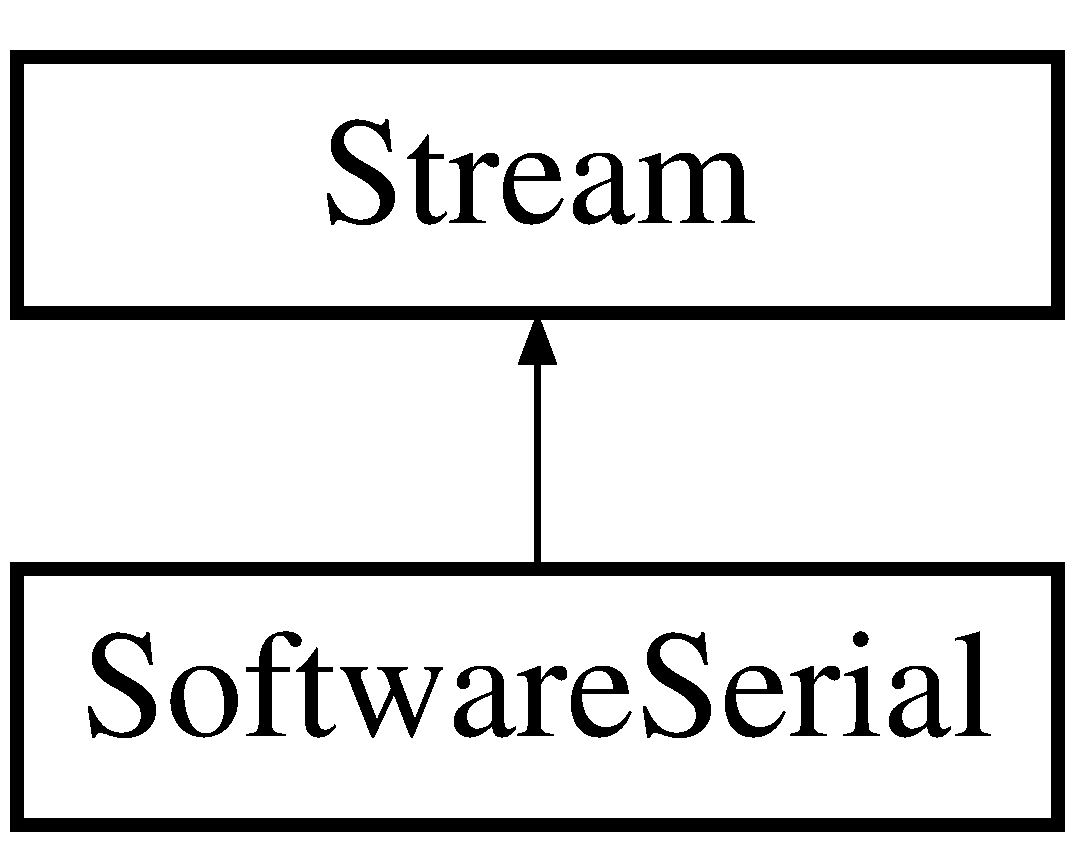
\includegraphics[height=2.000000cm]{class_software_serial}
\end{center}
\end{figure}
\subsection*{Public Member Functions}
\begin{DoxyCompactItemize}
\item 
\hypertarget{class_software_serial_aab36336db4a1ca5073071c07d910cb87}{}{\bfseries Software\+Serial} (uint8\+\_\+t receive\+Pin, uint8\+\_\+t transmit\+Pin, bool inverse\+\_\+logic=false)\label{class_software_serial_aab36336db4a1ca5073071c07d910cb87}

\item 
\hypertarget{class_software_serial_af1b194359d70894b3a2f38236a68480e}{}void {\bfseries begin} (long speed)\label{class_software_serial_af1b194359d70894b3a2f38236a68480e}

\item 
\hypertarget{class_software_serial_ad235539ef28939836bd0bde9387eb8fc}{}bool {\bfseries listen} ()\label{class_software_serial_ad235539ef28939836bd0bde9387eb8fc}

\item 
\hypertarget{class_software_serial_a9034270f7de617b3cc7d3f38f3a8e0df}{}void {\bfseries end} ()\label{class_software_serial_a9034270f7de617b3cc7d3f38f3a8e0df}

\item 
\hypertarget{class_software_serial_a7b3fb4a8f57d2b5f2233f841d71ef80f}{}bool {\bfseries is\+Listening} ()\label{class_software_serial_a7b3fb4a8f57d2b5f2233f841d71ef80f}

\item 
\hypertarget{class_software_serial_ac6d4d5dfbe05515bf23766e2c8abfd46}{}bool {\bfseries overflow} ()\label{class_software_serial_ac6d4d5dfbe05515bf23766e2c8abfd46}

\item 
\hypertarget{class_software_serial_a51c2d2e79f0d982b1ef9cc9ac4453648}{}int {\bfseries peek} ()\label{class_software_serial_a51c2d2e79f0d982b1ef9cc9ac4453648}

\item 
\hypertarget{class_software_serial_ac24e5c6af203ec636c0a200b0cb3caf0}{}virtual size\+\_\+t {\bfseries write} (uint8\+\_\+t byte)\label{class_software_serial_ac24e5c6af203ec636c0a200b0cb3caf0}

\item 
\hypertarget{class_software_serial_a2d0b2f2868d519c716114777f482705b}{}virtual int {\bfseries read} ()\label{class_software_serial_a2d0b2f2868d519c716114777f482705b}

\item 
\hypertarget{class_software_serial_a4cbf77a4e90e15ca576972d7952659c5}{}virtual int {\bfseries available} ()\label{class_software_serial_a4cbf77a4e90e15ca576972d7952659c5}

\item 
\hypertarget{class_software_serial_a9a46db376a19fc958e011e38799b902c}{}virtual void {\bfseries flush} ()\label{class_software_serial_a9a46db376a19fc958e011e38799b902c}

\end{DoxyCompactItemize}
\subsection*{Static Public Member Functions}
\begin{DoxyCompactItemize}
\item 
\hypertarget{class_software_serial_a1546972033f250750ffd731dd15acfdf}{}static void {\bfseries handle\+\_\+interrupt} ()\label{class_software_serial_a1546972033f250750ffd731dd15acfdf}

\end{DoxyCompactItemize}


The documentation for this class was generated from the following files\+:\begin{DoxyCompactItemize}
\item 
Arduino\+Libraries/\+Software\+Serial/Software\+Serial.\+h\item 
Arduino\+Libraries/\+Software\+Serial/Software\+Serial.\+cpp\end{DoxyCompactItemize}

\hypertarget{class_s_p_i_class}{}\section{S\+P\+I\+Class Class Reference}
\label{class_s_p_i_class}\index{S\+P\+I\+Class@{S\+P\+I\+Class}}
\subsection*{Static Public Member Functions}
\begin{DoxyCompactItemize}
\item 
\hypertarget{class_s_p_i_class_a821dccd5dda20ccd9093fc35cce74ae5}{}static byte {\bfseries transfer} (byte \+\_\+data)\label{class_s_p_i_class_a821dccd5dda20ccd9093fc35cce74ae5}

\item 
\hypertarget{class_s_p_i_class_a715dff0f3f87dbb64b2ef83d15ee97c0}{}static void {\bfseries attach\+Interrupt} ()\label{class_s_p_i_class_a715dff0f3f87dbb64b2ef83d15ee97c0}

\item 
\hypertarget{class_s_p_i_class_abf83d2ea70e46aed0dd278011e1e8741}{}static void {\bfseries detach\+Interrupt} ()\label{class_s_p_i_class_abf83d2ea70e46aed0dd278011e1e8741}

\item 
\hypertarget{class_s_p_i_class_a4a2646959a242f6af423b04734c003f0}{}static void {\bfseries begin} ()\label{class_s_p_i_class_a4a2646959a242f6af423b04734c003f0}

\item 
\hypertarget{class_s_p_i_class_a79d89d8e3f5f1b003cb7b0aed2d77eab}{}static void {\bfseries end} ()\label{class_s_p_i_class_a79d89d8e3f5f1b003cb7b0aed2d77eab}

\item 
\hypertarget{class_s_p_i_class_aa50f88614cda319d2d983749b9a7626d}{}static void {\bfseries set\+Bit\+Order} (uint8\+\_\+t)\label{class_s_p_i_class_aa50f88614cda319d2d983749b9a7626d}

\item 
\hypertarget{class_s_p_i_class_ae7e89ec7f26a6412fb2d218db331195d}{}static void {\bfseries set\+Data\+Mode} (uint8\+\_\+t)\label{class_s_p_i_class_ae7e89ec7f26a6412fb2d218db331195d}

\item 
\hypertarget{class_s_p_i_class_ac364a8e46c27d1f6d94a58e9a2455c62}{}static void {\bfseries set\+Clock\+Divider} (uint8\+\_\+t)\label{class_s_p_i_class_ac364a8e46c27d1f6d94a58e9a2455c62}

\end{DoxyCompactItemize}


The documentation for this class was generated from the following files\+:\begin{DoxyCompactItemize}
\item 
Arduino\+Libraries/\+S\+P\+I/S\+P\+I.\+h\item 
Arduino\+Libraries/\+S\+P\+I/S\+P\+I.\+cpp\end{DoxyCompactItemize}

\chapter{File Documentation}
\hypertarget{conf__board_8h}{}\section{src/config/conf\+\_\+board.h File Reference}
\label{conf__board_8h}\index{src/config/conf\+\_\+board.\+h@{src/config/conf\+\_\+board.\+h}}


A\+Tmega2560 on S\+T\+K600 board configuration template.  




\subsection{Detailed Description}
A\+Tmega2560 on S\+T\+K600 board configuration template. 


%--- End generated contents ---

% Index
\backmatter
\newpage
\phantomsection
\clearemptydoublepage
\addcontentsline{toc}{chapter}{Index}
\printindex

\end{document}
